        %%******************************************%%
        %%                                          %%
        %%        Modello di tesi di laurea         %%
        %%            di Andrea Giraldin            %%
        %%                                          %%
        %%             2 novembre 2012              %%
        %%                                          %%
        %%******************************************%%


% I seguenti commenti speciali impostano:
% 1. 
% 2. PDFLaTeX come motore di composizione;
% 3. tesi.tex come documento principale;
% 4. il controllo ortografico italiano per l'editor.

% !TEX encoding = UTF-8
% !TEX TS-program = pdflatex
% !TEX root = tesi.tex
% !TEX spellcheck = it-IT

\documentclass[10pt,                    % corpo del font principale
               a4paper,                 % carta A4
               twoside,                 % impagina per fronte-retro
               openright,               % inizio capitoli a destra
               english,                 
               italian,                 
               ]{book}    

%**************************************************************
% Importazione package
%************************************************************** 

%\usepackage{amsmath,amssymb,amsthm}    % matematica

\usepackage[T1]{fontenc}                % codifica dei font:
                                        % NOTA BENE! richiede una distribuzione *completa* di LaTeX

\usepackage[utf8]{inputenc}             % codifica di input; anche [latin1] va bene
                                        % NOTA BENE! va accordata con le preferenze dell'editor

\usepackage[english, italian]{babel}    % per scrivere in italiano e in inglese;
                                        % l'ultima lingua (l'italiano) risulta predefinita

\usepackage{bookmark}                   % segnalibri

\usepackage{caption}                    % didascalie

\usepackage{chngpage,calc}              % centra il frontespizio

\usepackage{csquotes}                   % gestisce automaticamente i caratteri (")

\usepackage{emptypage}                  % pagine vuote senza testatina e piede di pagina

\usepackage{epigraph}			% per epigrafi

\usepackage{eurosym}                    % simbolo dell'euro

%\usepackage{indentfirst}               % rientra il primo paragrafo di ogni sezione

\usepackage{graphicx}                   % immagini

\usepackage{hyperref}                   % collegamenti ipertestuali

\usepackage[binding=5mm]{layaureo}      % margini ottimizzati per l'A4; rilegatura di 5 mm

\usepackage{listings}                   % codici

\usepackage{microtype}                  % microtipografia

\usepackage{mparhack,fixltx2e,relsize}  % finezze tipografiche

\usepackage{nameref}                    % visualizza nome dei riferimenti                                      

\usepackage[font=small]{quoting}        % citazioni

\usepackage{subfig}                     % sottofigure, sottotabelle

\usepackage[italian]{varioref}          % riferimenti completi della pagina

\usepackage[dvipsnames]{xcolor}         % colori

\usepackage{booktabs}                   % tabelle                                       
\usepackage{tabularx}                   % tabelle di larghezza prefissata                                    
\usepackage{longtable}                  % tabelle su più pagine                                        
\usepackage{ltxtable}                   % tabelle su più pagine e adattabili in larghezza

\usepackage[toc, acronym]{glossaries}   % glossario
                                        % per includerlo nel documento bisogna:
                                        % 1. compilare una prima volta tesi.tex;
                                        % 2. eseguire: makeindex -s tesi.ist -t tesi.glg -o tesi.gls tesi.glo
                                        % 3. eseguire: makeindex -s tesi.ist -t tesi.alg -o tesi.acr tesi.acn
                                        % 4. compilare due volte tesi.tex.

\usepackage[backend=biber,style=verbose-ibid,hyperref,backref]{biblatex}
                                        % eccellente pacchetto per la bibliografia; 
                                        % produce uno stile di citazione autore-anno; 
                                        % lo stile "numeric-comp" produce riferimenti numerici
                                        % per includerlo nel documento bisogna:
                                        % 1. compilare una prima volta tesi.tex;
                                        % 2. eseguire: biber tesi
                                        % 3. compilare ancora tesi.tex.

%**************************************************************
% file contenente le impostazioni della tesi
%**************************************************************

%**************************************************************
% Frontespizio
%**************************************************************

% Autore
\newcommand{\myName}{Stefano Zanatta}                                    
\newcommand{\myTitle}{Analisi e sviluppo di un'applicazione per la configurazione automatica di una chatbot professionale}
\newcommand{\company}{PAT s.r.l}
% Tipo di tesi                   
\newcommand{\myDegree}{Tesi di laurea triennale}

% Università             
\newcommand{\myUni}{Università degli Studi di Padova}

% Facoltà       
\newcommand{\myFaculty}{Corso di Laurea in Informatica}

% Dipartimento
\newcommand{\myDepartment}{Dipartimento di Matematica "Tullio Levi-Civita"}

% Titolo del relatore
\newcommand{\profTitle}{Prof.}

% Relatore
\newcommand{\myProf}{Ballan Lamberto}

% Luogo
\newcommand{\myLocation}{Padova}

% Anno accademico
\newcommand{\myAA}{2018-2019}

% Data discussione
\newcommand{\myTime}{Settembre 2019}

\newcommand{\app}{NLP Generator}


%**************************************************************
% Impostazioni di impaginazione
% see: http://wwwcdf.pd.infn.it/AppuntiLinux/a2547.htm
%**************************************************************

\setlength{\parindent}{14pt}   % larghezza rientro della prima riga
\setlength{\parskip}{0pt}   % distanza tra i paragrafi


%**************************************************************
% Impostazioni di biblatex
%**************************************************************
\bibliography{bibliografia} % database di biblatex 

\defbibheading{bibliography} {
    \cleardoublepage
    \phantomsection 
    \addcontentsline{toc}{chapter}{\bibname}
    \chapter*{\bibname\markboth{\bibname}{\bibname}}
}

\setlength\bibitemsep{1.5\itemsep} % spazio tra entry

\DeclareBibliographyCategory{opere}
\DeclareBibliographyCategory{web}

\addtocategory{opere}{womak:lean-thinking}
\addtocategory{web}{site:agile-manifesto}

\defbibheading{opere}{\section*{Riferimenti bibliografici}}
\defbibheading{web}{\section*{Siti Web consultati}}


%**************************************************************
% Impostazioni di caption
%**************************************************************
\captionsetup{
    tableposition=top,
    figureposition=bottom,
    font=small,
    format=hang,
    labelfont=bf
}

%**************************************************************
% Impostazioni di glossaries
%**************************************************************

%**************************************************************
% Acronimi
%**************************************************************
\renewcommand{\acronymname}{Acronimi e abbreviazioni}

\newacronym[description={\glslink{apig}{Application Program Interface}}]
    {api}{API}{Application Program Interface}

\newacronym[description={\glslink{umlg}{Unified Modeling Language}}]
    {uml}{UML}{Unified Modeling Language}

%**************************************************************
% Glossario
%**************************************************************
%\renewcommand{\glossaryname}{Glossario}

\newglossaryentry{apig}
{
    name=\glslink{api}{API},
    text=Application Program Interface,
    sort=api,
    description={in informatica con il termine \emph{Application Programming Interface API} (ing. interfaccia di programmazione di un'applicazione) si indica ogni insieme di procedure disponibili al programmatore, di solito raggruppate a formare un set di strumenti specifici per l'espletamento di un determinato compito all'interno di un certo programma. La finalità è ottenere un'astrazione, di solito tra l'hardware e il programmatore o tra software a basso e quello ad alto livello semplificando così il lavoro di programmazione}
}

\newglossaryentry{umlg}
{
    name=\glslink{uml}{UML},
    text=UML,
    sort=uml,
    description={in ingegneria del software \emph{UML, Unified Modeling Language} (ing. linguaggio di modellazione unificato) è un linguaggio di modellazione e specifica basato sul paradigma object-oriented. L'\emph{UML} svolge un'importantissima funzione di ``lingua franca'' nella comunità della progettazione e programmazione a oggetti. Gran parte della letteratura di settore usa tale linguaggio per descrivere soluzioni analitiche e progettuali in modo sintetico e comprensibile a un vasto pubblico}
}
 % database di termini
\makeglossaries


%**************************************************************
% Impostazioni di graphicx
%**************************************************************
\graphicspath{{immagini/}} % cartella dove sono riposte le immagini


%**************************************************************
% Impostazioni di hyperref
%**************************************************************
\hypersetup{
    %hyperfootnotes=false,
    %pdfpagelabels,
    %draft,	% = elimina tutti i link (utile per stampe in bianco e nero)
    colorlinks=true,
    linktocpage=true,
    pdfstartpage=1,
    pdfstartview=FitV,
    % decommenta la riga seguente per avere link in nero (per esempio per la stampa in bianco e nero)
    %colorlinks=false, linktocpage=false, pdfborder={0 0 0}, pdfstartpage=1, pdfstartview=FitV,
    breaklinks=true,
    pdfpagemode=UseNone,
    pageanchor=true,
    pdfpagemode=UseOutlines,
    plainpages=false,
    bookmarksnumbered,
    bookmarksopen=true,
    bookmarksopenlevel=1,
    hypertexnames=true,
    pdfhighlight=/O,
    %nesting=true,
    %frenchlinks,
    urlcolor=webbrown,
    linkcolor=RoyalBlue,
    citecolor=webgreen,
    %pagecolor=RoyalBlue,
    %urlcolor=Black, linkcolor=Black, citecolor=Black, %pagecolor=Black,
    pdftitle={\myTitle},
    pdfauthor={\textcopyright\ \myName, \myUni, \myFaculty},
    pdfsubject={},
    pdfkeywords={},
    pdfcreator={pdfLaTeX},
    pdfproducer={LaTeX}
}

%**************************************************************
% Impostazioni di itemize
%**************************************************************
\renewcommand{\labelitemi}{$\ast$}

%\renewcommand{\labelitemi}{$\bullet$}
%\renewcommand{\labelitemii}{$\cdot$}
%\renewcommand{\labelitemiii}{$\diamond$}
%\renewcommand{\labelitemiv}{$\ast$}


%**************************************************************
% Impostazioni di listings
%**************************************************************
\lstset{
    language=[LaTeX]Tex,%C++,
    keywordstyle=\color{RoyalBlue}, %\bfseries,
    basicstyle=\small\ttfamily,
    %identifierstyle=\color{NavyBlue},
    commentstyle=\color{Green}\ttfamily,
    stringstyle=\rmfamily,
    numbers=none, %left,%
    numberstyle=\scriptsize, %\tiny
    stepnumber=5,
    numbersep=8pt,
    showstringspaces=false,
    breaklines=true,
    frameround=ftff,
    frame=single
} 


%**************************************************************
% Impostazioni di xcolor
%**************************************************************
\definecolor{webgreen}{rgb}{0,.5,0}
\definecolor{webbrown}{rgb}{.6,0,0}


%**************************************************************
% Altro
%**************************************************************

\newcommand{\omissis}{[\dots\negthinspace]} % produce [...]

% eccezioni all'algoritmo di sillabazione
\hyphenation
{
    ma-cro-istru-zio-ne
    gi-ral-din
}

\newcommand{\sectionname}{sezione}
\addto\captionsitalian{\renewcommand{\figurename}{Figura}
                       \renewcommand{\tablename}{Tabella}}

\newcommand{\glsfirstoccur}{\ap{{[g]}}}

\newcommand{\intro}[1]{\emph{\textsf{#1}}}

%**************************************************************
% Environment per ``rischi''
%**************************************************************
\newcounter{riskcounter}                % define a counter
\setcounter{riskcounter}{0}             % set the counter to some initial value

%%%% Parameters
% #1: Title
\newenvironment{risk}[1]{
    \refstepcounter{riskcounter}        % increment counter
    \par \noindent                      % start new paragraph
    \textbf{\arabic{riskcounter}. #1}   % display the title before the 
                                        % content of the environment is displayed 
}{
    \par\medskip
}

\newcommand{\riskname}{Rischio}

\newcommand{\riskdescription}[1]{\textbf{\\Descrizione:} #1.}

\newcommand{\risksolution}[1]{\textbf{\\Soluzione:} #1.}

%**************************************************************
% Environment per ``use case''
%**************************************************************
\newcounter{usecasecounter}             % define a counter
\setcounter{usecasecounter}{0}          % set the counter to some initial value

%%%% Parameters
% #1: ID
% #2: Nome
\newenvironment{usecase}[2]{
    \renewcommand{\theusecasecounter}{\usecasename #1}  % this is where the display of 
                                                        % the counter is overwritten/modified
    \refstepcounter{usecasecounter}             % increment counter
    \vspace{10pt}
    \par \noindent                              % start new paragraph
    {\large \textbf{\usecasename #1: #2}}       % display the title before the 
                                                % content of the environment is displayed 
    \medskip
}{
    \medskip
}

\newcommand{\usecasename}{UC}

\newcommand{\usecaseactors}[1]{\textbf{\\Attori Principali:} #1. \vspace{4pt}}
\newcommand{\usecasepre}[1]{\textbf{\\Precondizioni:} #1. \vspace{4pt}}
\newcommand{\usecasedesc}[1]{\textbf{\\Descrizione:} #1. \vspace{4pt}}
\newcommand{\usecasepost}[1]{\textbf{\\Postcondizioni:} #1. \vspace{4pt}}
\newcommand{\usecasealt}[1]{\textbf{\\Scenario Alternativo:} #1. \vspace{4pt}}

%**************************************************************
% Environment per ``namespace description''
%**************************************************************

\newenvironment{namespacedesc}{
    \vspace{10pt}
    \par \noindent                              % start new paragraph
    \begin{description} 
}{
    \end{description}
    \medskip
}

\newcommand{\classdesc}[2]{\item[\textbf{#1:}] #2}                     % file con le impostazioni personali

\begin{document}
%**************************************************************
% Materiale iniziale
%**************************************************************
\frontmatter
% !TEX encoding = UTF-8
% !TEX TS-program = pdflatex
% !TEX root = ../tesi.tex

%**************************************************************
% Frontespizio 
%**************************************************************
\begin{titlepage}

\begin{center}

\begin{LARGE}
\textbf{\myUni}\\
\end{LARGE}

\vspace{10pt}

\begin{Large}
\textsc{\myDepartment}\\
\end{Large}

\vspace{10pt}

\begin{large}
\textsc{\myFaculty}\\
\end{large}

\vspace{30pt}
\begin{figure}[htbp]
\begin{center}

\includegraphics[height=6cm]{logo-unipd}
\end{center}
\end{figure}
\vspace{30pt} 

\begin{LARGE}
\begin{center}
\textbf{\myTitle}\\
\end{center}
\end{LARGE}

\vspace{10pt} 

\begin{large}
\textsl{\myDegree}\\
\end{large}

\vspace{40pt} 

\begin{large}
\begin{flushleft}
\textit{Relatore}\\ 
\vspace{5pt} 
\profTitle \myProf
\end{flushleft}

\vspace{0pt} 

\begin{flushright}
\textit{Laureando}\\ 
\vspace{5pt} 
\myName
\end{flushright}
\end{large}

\vspace{40pt}

\line(1, 0){338} \\
\begin{normalsize}
\textsc{Anno Accademico \myAA}
\end{normalsize}

\end{center}
\end{titlepage} 
% !TEX encoding = UTF-8
% !TEX TS-program = pdflatex
% !TEX root = ../tesi.tex

%**************************************************************
% Colophon
%**************************************************************
\clearpage
\phantomsection
\thispagestyle{empty}

\hfill

\vfill

\noindent\myName: \textit{\myTitle,}
\myDegree,
\textcopyright\ \myTime.
% !TEX encoding = UTF-8
% !TEX TS-program = pdflatex
% !TEX root = ../tesi.tex

%**************************************************************
% Dedica
%**************************************************************
\cleardoublepage
\phantomsection
\thispagestyle{empty}
\pdfbookmark{Dedica}{Dedica}

\vspace*{3cm}

\begin{center}
Lorem ipsum dolor sit amet, consectetuer adipiscing elit. \\ \medskip
--- Oscar Wilde    
\end{center}

\medskip

\begin{center}
Dedicato a ...
\end{center}

% !TEX encoding = UTF-8
% !TEX TS-program = pdflatex
% !TEX root = ../tesi.tex

%**************************************************************
% Sommario
%**************************************************************
\cleardoublepage
\phantomsection
\pdfbookmark{Sommario}{Sommario}
\begingroup
\let\clearpage\relax
\let\cleardoublepage\relax
\let\cleardoublepage\relax

\chapter*{Sommario}

Il presente documento descrive il lavoro svolto durante il periodo di stage, della durata di trecentododici ore, dal laureando Stefano Zanatta presso l'azienda {\company}. Gli obbiettivi principali del progetto erano:
\begin{itemize}
    \item studio del motore semantico di Engagent, la chatbot professionale dell'azienda;
    \item studio dei risultati di un algoritmo di clustering, sviluppato da ricercatori esterni all'azienda;
    \item integrazione automatica dei cluster con Engagent, eseguendo operazioni di pos-tagging.
\end{itemize}

%\vfill
%
%\selectlanguage{english}
%\pdfbookmark{Abstract}{Abstract}
%\chapter*{Abstract}
%
%\selectlanguage{italian}

\endgroup			

\vfill


% !TEX encoding = UTF-8
% !TEX TS-program = pdflatex
% !TEX root = ../tesi.tex

%**************************************************************
% Ringraziamenti
%**************************************************************
\cleardoublepage
\phantomsection
\pdfbookmark{Ringraziamenti}{ringraziamenti}
\begin{flushright}{
	\slshape    
	``Life is really simple, but we insist on making it complicated''} \\ 
	\medskip
    --- Confucius
\end{flushright}


\bigskip

\begingroup
\let\clearpage\relax
\let\cleardoublepage\relax
\let\cleardoublepage\relax

\chapter*{Ringraziamenti}

\noindent \textit{Innanzitutto, vorrei ringrazione il Prof. Lamberto Ballan, relatore della mia tesi, per l'aiuto e il sostegno fornitomi durante la stesura della tesi.}\\
\noindent \textit{Vorrei ringraziare il tutor aziendale Davide Bastianetto, per avermi dato l'opportunità di svolgere lo stage a PAT.}\\
\noindent \textit{Desidero ringraziare con affetto i miei genitori e mio fratello per il sostegno morale (ed economico) dimostratomi durante questi anni.}\\

\bigskip

\noindent\textit{\myLocation, \myTime}
\hfill \myName

\endgroup


% !TEX encoding = UTF-8
% !TEX TS-program = pdflatex
% !TEX root = ../tesi.tex

%**************************************************************
% Indici
%**************************************************************
\cleardoublepage
\pdfbookmark{\contentsname}{tableofcontents}
\setcounter{tocdepth}{2}
\tableofcontents
%\markboth{\contentsname}{\contentsname} 
\clearpage

\begingroup 
    \let\clearpage\relax
    \let\cleardoublepage\relax
    \let\cleardoublepage\relax
    %*******************************************************
    % Elenco delle figure
    %*******************************************************    
    \phantomsection
    \pdfbookmark{\listfigurename}{lof}
    \listoffigures

    \vspace*{8ex}

    %*******************************************************
    % Elenco delle tabelle
    %*******************************************************
    \phantomsection
    \pdfbookmark{\listtablename}{lot}
    \listoftables
        
    \vspace*{8ex}
\endgroup

\cleardoublepage

\cleardoublepage

%**************************************************************
% Materiale principale
%**************************************************************
\mainmatter
% !TEX encoding = UTF-8
% !TEX TS-program = pdflatex
% !TEX root = ../tesi.tex

%**************************************************************
\chapter{Introduzione}
\label{cap:introduzione}
%**************************************************************
\section{L'azienda}

\company è un'azienda italiana che da 25 anni sviluppa soluzioni software per altre aziende e privati.\\
L'azienda lavora su 5 diversi macro-progetti, uno dei quali è Engagent, la chatbot professionale oggetto dei miei due mesi di stage.\\
Dal 2013, PAT è entrata a far parte di Zucchetti Group.

\subsection{Prodotti e servizi}
L'azienda offre ai suoi clienti l'automatizzazione dei processi e il miglioramento dell'\textit{user experience} dei loro prodotti.
PAT concretizza quesi obbiettivi attraverso i seguenti prodotti:
\begin{itemize}
    \item Engagent: chatbot semi-automatizzata per uso professionale; 
    \item Helpdesk;
    \item Infinite: \textit{CRM} software orientato alla relazione tra cliente e azienda;
    \item Brain \textit{Interactive}: piattaforma per governare dei servizi personalizzati attraverso dei diagrammi di flusso; 
    \item Teammee: piattaforma per la comunicazione tra i dipendenti in un'azienda, usando la logica dei social networks;
\end{itemize}

\subsubsection{Engagent}
Engagent è una chatbot orientata al business, con un agente virtuale integrato.\\
In \textit{backend}, un motore semantico permette di capire cosa sta chiedendo l'utente e trovare la risposta più coerente. Se la domanda è troppo complessa, il motore semantico estrate la categoria della domanda e la reinderizza all'operatore (umano) adeguato.\\

\subsection{Organizzazione e Metodo di lavoro}
L'azienda è divisa in più gruppi di lavoro, uno per ogni macro-progetto, oltre alla segreteria e direzione.\\
Ogni team è separato dagli altri, anche se la collaborazione tra le parti è molto presente.\\
Tutti i team di sviluppo in \company seguono una metodologia Agile. Questa metodologia fa parte delle metodologie iterative. Le brevi iterazioni (o sprint, di circa 3-4 settimane) sono seguite dalla \textit{review} del lavoro svolto. Il focus principale si trova nel cliente, difatti ci deve essere una interazione costante per capire quali sono le \textit{feature} più importanti, ovvero quelli da sviluppare prima.\\
Il team a cui ho preso parte segue correttamente questa metodologia: il contatto con il cliente è giornaliero, che sia manutenzione o nuove \textit{features} da sviluppare.
%**************************************************************
\section{Obbiettivi personali}

Volevo contribuire a un progetto software in ambito professionale, facendo contemporaneamente i primi passi nel mondo delle intelligenze artificiali.\\
Il progetto proposto da PAT racchiudeva queste prerogative: sarei stato inserito in un progetto maturo e, con l'aiuto di esperti nel settore, avrei potuto lavorare con un algoritmo di clustering.   

%**************************************************************
\section{Organizzazione del testo}

\begin{description}
    \item[{\hyperref[cap:processi-metodologie]{Il secondo capitolo}}] descrive i processi e le metodologie utilizzate durante lo stage;
    
    \item[{\hyperref[cap:descrizione-stage]{Il terzo capitolo}}] approfondisce i lati meno tecnici dello stage; 
    
    \item[{\hyperref[cap:analisi-requisiti]{Il quarto capitolo}}] approfondisce nel dettaglio i requisiti del progetto, descrivendo il processo di analisi che ha portato alla loro stesura;
    
    \item[{\hyperref[cap:progettazione-codifica]{Il quinto capitolo}}] approfondisce l'architettura del software sviluppato, con il supporto di esempi specifici e schemi ad alto livello;
    
    \item[{\hyperref[cap:verifica-validazione]{Il sesto capitolo}}] approfondisce le tecniche di verifica e validazione utilizzate durante lo stage, con i relativi risultati;
    
    \item[{\hyperref[cap:conclusioni]{Nel settimo capitolo}}] contiene il resoconto dello stage. 
\end{description}

Riguardo la stesura del testo, relativamente al documento sono state adottate le seguenti convenzioni tipografiche:
\begin{itemize}
	\item gli acronimi, le abbreviazioni e i termini ambigui o di uso non comune menzionati vengono definiti nel glossario, situato alla fine del presente documento;
	\item per la prima occorrenza dei termini riportati nel glossario viene utilizzata la seguente nomenclatura: \emph{parola}\glsfirstoccur;
	\item i termini in lingua straniera o facenti parti del gergo tecnico sono evidenziati con il carattere \emph{corsivo}.
\end{itemize}             % Introduzione
% !TEX encoding = UTF-8
% !TEX TS-program = pdflatex
% !TEX root = ../tesi.tex

%**************************************************************
\chapter{Descrizione dello stage}
\label{cap:descrizione-stage}

%**************************************************************
\section{Il progetto}\label{sec:progetto}

Il progetto è nato dalla necessità dell'azienda \company{} di automatizzare il processo di configurazione del motore semantico di \gls{Engagent}\glsfirstoccur{}, il quale richiede la creazione manuale di \emph{synset}\glsfirstoccur{} e \emph{regole}\glsfirstoccur{}. Questo processo è economicamente fattibile e vantaggioso finché le dimensioni delle regole create sono ridotte, ma il costo cresce esponenzialmente con l'aumentare delle regole.\\
Più regole rendono più precisa la chatbot, ma incrementano di conseguenza i \gls{synset}\glsfirstoccur{} da inserire, prolungando i tempi di compilazione dell'\emph{NLP}\glsfirstoccur{} da qualche giorno a settimane.

%**************************************************************
\section{Obiettivi Aziendali}
L'obiettivo di automatizzare il processo di configurazione di Engagent non è nato con il progetto di stage, ma qualche anno fa, mentre il \textit{Machine Learning} diventava sempre più popolare. \company{} attribuì questo compito a un team esterno. Il loro compito consisteva nell'implementazione di un algoritmo di \textit{ML}, per la generazione di cluster contenenti gli ingredienti essenziali alla configurazione di Engagent.
Verso l'inizio dell'anno, i progressi fatti da questo team erano convincenti, quindi \company{} aveva l'intenzione di sperimentare l'integrazione di tali risultati con il proprio sistema.\\
Dallo stage, l'azienda si aspettava i seguenti prodotti:
\begin{itemize}
    \item \textbf{Studio di fattibilità:} analisi del problema\riferimento{cap:analisi-requisiti} e \gls{scouting}\glsfirstoccur{} di soluzioni già esistenti;
    \item \textbf{\app{}:} un'applicazione per la creazione del modello per il motore semantico di Engagent;
    \item \textbf{manuale:} manuale tecnico per l'utilizzo e la manutenzione dell'applicazione.    
\end{itemize}
%**************************************************************
\section{Obiettivi personali}

Durante la ricerca dell'azienda per lo stage, volevo contribuire a un progetto software in ambito professionale, facendo contemporaneamente i primi passi nel mondo delle intelligenze artificiali.\\
Il progetto proposto da PAT racchiudeva queste prerogative: sarei stato inserito in un progetto maturo e, con l'aiuto di esperti nel settore, avrei potuto lavorare con degli algoritmi di clustering.   

%**************************************************************
\section{Pianificazione}

Con l'aiuto del tutor aziendale, ho redatto il piano di lavoro, che comprende 312 ore distribuite in 8 ore al giorno, per 5 giorni alla settimana (lunedì 24 luglio mi sono dovuto assentare da lavoro, con il consenso del tutor aziendale, per un esame universitario).\\
La pianificazione ha avuto delle modifiche durante l'avanzare del progetto, vista la sua natura "sperimentale". Per esempio, il linguaggio di programmazione Python è stato accordato assieme al tutor aziendale solamente dopo un'analisi approfondita del problema.
Di seguito viene riportata l'ultima versione del piano di lavoro.
\begin{itemize}
    \item \textbf{I settimana:}
    \begin{itemize}
        \item studio della piattaforma \emph{Engagent};
    \end{itemize}
    \item \textbf{II settimana:}
    \begin{itemize}
        \item analisi e stesura di un report, riguardante il problema della creazione automatica del file di configurazione\riferimento{sec:progetto};
        \item preparazione dell'ambiente di lavoro;
    \end{itemize}
    \item \textbf{III settimana:}
        \begin{itemize}
            \item ricerca e sperimentazione di possibili soluzioni già esistenti per automatizzare la generazione di sinonimi;
            \item analisi e progettazione (al alto livello) di \app{};
            \item progettazione di dettaglio e implementazione del model\riferimento{sec:progettazione:model};
        \end{itemize}
    \item \textbf{IV settimana:}
    \begin{itemize}
        \item implementazione di \app{};
        \item stesura di test di unità;
    \end{itemize}
    \item \textbf{V settimana:}
    \begin{itemize}
        \item implementazione e miglioramento delle prestazioni di \emph{\app{}};
        \item verifica dei risultati di \emph{\app{}} da parte del tutor aziendale;
    \end{itemize}
    \item \textbf{VI settimana:}
    \begin{itemize}
        \item analisi per il miglioramento dei risultati di \emph{\app{}}
        \item progettazione di dettaglio e implementazione;
        \item documentazione;
    \end{itemize}
    \item \textbf{VII settimana:}
    \begin{itemize}
        \item documentazione e validazione;
    \end{itemize}
    \item \textbf{VIII settimana:}
    \begin{itemize}
        \item collaudo.
    \end{itemize}
\end{itemize}
             % Processi
% !TEX encoding = UTF-8
% !TEX TS-program = pdflatex
% !TEX root = ../tesi.tex

%**************************************************************
\chapter{Analisi dei requisiti}
\label{cap:analisi-requisiti}

%**************************************************************

\section{Casi d'uso}
La progettazione dell'applicazione è iniziata con la stesura dei casi d'uso, supportati da diagrammi dei casi d'uso coerenti con lo standard UML.\\
I casi d'uso sono aumentati durante tutta la durata dello stage. Durante lo sviluppo, assieme al tutor, individuavamo nuove funzionalità per migliorare i risultati e aumentare l'automazione.

\begin{usecase}{0}{Scenario principale}
\usecaseactors{Utente}
\usecasepre{Il sistema è stato installato correttamente. L'utente ha aperto una \textit{shell} posizionata nella root dell'applicazione. (stato principale del sistema)}
\usecasedesc{Il sistema, tramite CLI (\textit{command line interface}), permette di:
    \begin{itemize}
        \item 1 inserire un file json;
        \item 2 inserire un file xmlsx;
        \item 3 personalizzare i parametri in output;
        \item 4 attivare o disattivare le funzionalità del programma;
        \item 5 creare una configurazione per il motore semantico di Engagent;
        \item 6 caricare automaticamente l'output in Engagent; 
        \item 7 inserire in input una configurazione già esistente;
        \item 8 utilizzo dell'applicazione attraverso una \textit{REST API};
        \item 9 visualizzazione delle informazione di esecuzione del sistema (\textit{log}).
    \end{itemize}
}
\begin{figure}[H]
    \centering 
    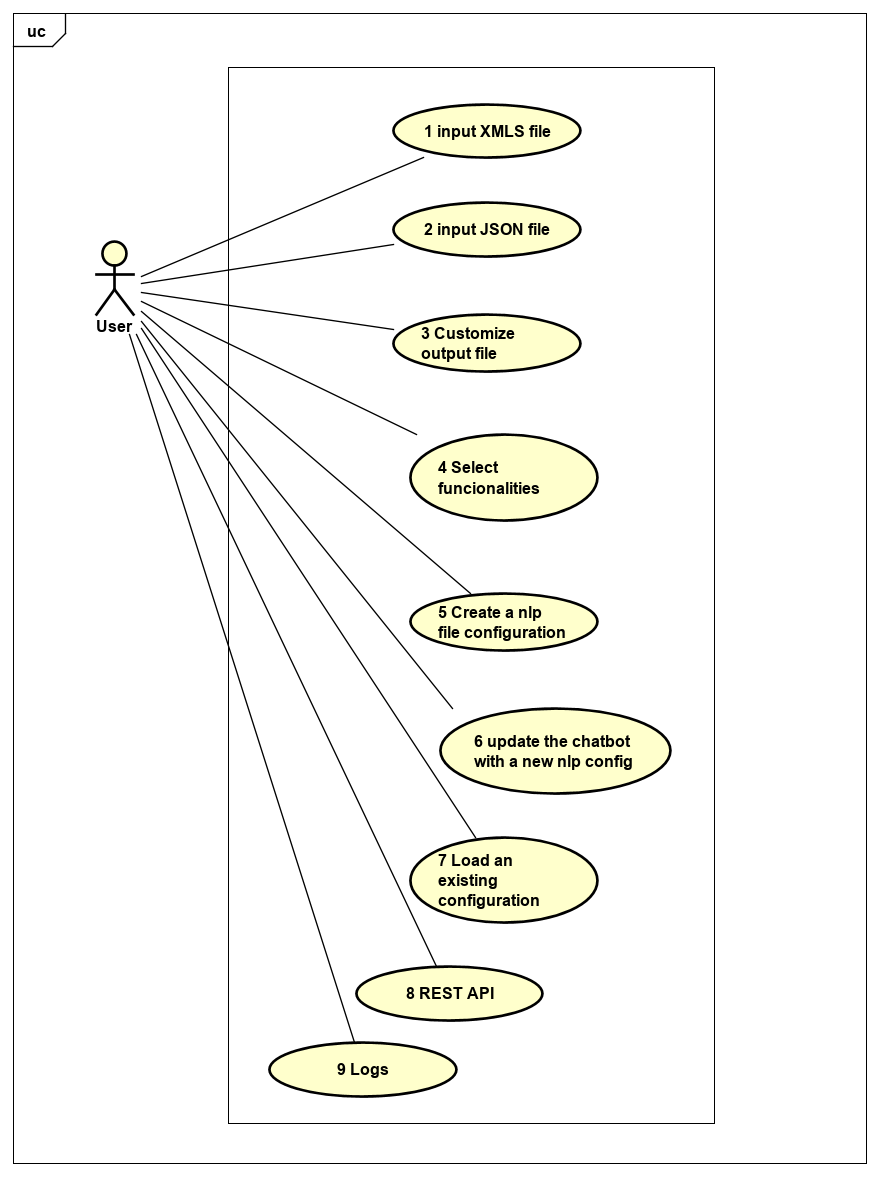
\includegraphics[width=0.9\columnwidth]{usecase/general_view.png} 
    \caption{Use Case - UC0: Scenario principale}
\end{figure}

\usecasepost{Il sistema è pronto per una nuova iterazione}
\label{uc:scenario-principale}
\end{usecase}

\begin{usecase}{1/2}{inserire un file json/xmlsx}
    \usecaseactors{Utente}
    \usecasepre{Il sistema mette a disposizione un comando per l'input di un file json/xmlsx}
    \usecasedesc{L'utente, tramite CLI, inserisce un file json/xmlsx}
    \usecasepost{Il sistema permette di inserire un nuovo file in input}
    \label{uc:1/2}
\end{usecase}

\begin{usecase}{3}{Personalizzazione parametri in output}
    \usecaseactors{Utente}
    \usecasepre{Il sistema mette a disposizione dei comandi per la personalizzazione dell'output}
    \usecasedesc{L'utente, tramite CLI, personalizza i parametri di output:
    \begin{itemize}
        \item 3.1 dominio;
        \item 3.2 lingua;
        \item 3.3 prefissi;
        \item 3.4 priorità delle regole.
    \end{itemize}
    }
    \usecasepost{Il sistema torna allo stato principale}
    \label{uc:3}
\end{usecase}

\begin{figure}[H]
    \centering 
    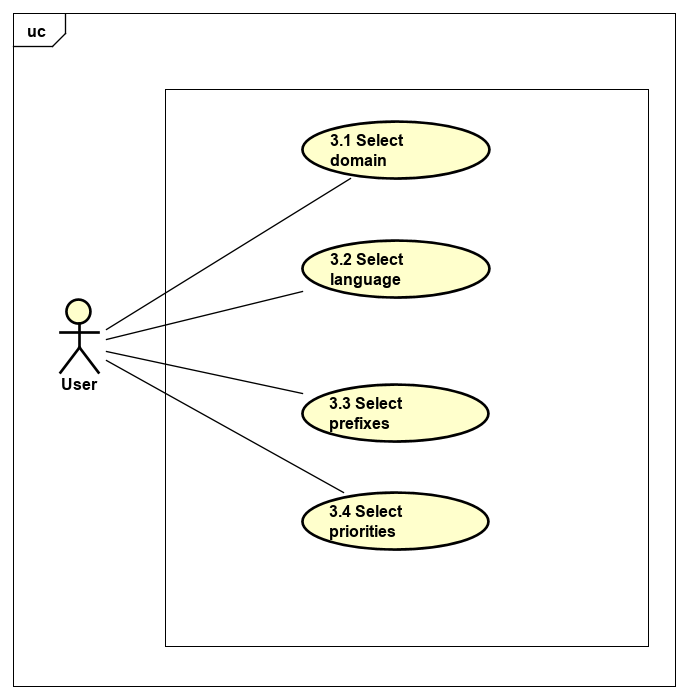
\includegraphics[width=0.9\columnwidth]{usecase/customize_output.png} 
    \caption{Use Case - UC3: Personalizzazione parametri in output}
\end{figure}

\begin{usecase}{3.1, 3.2, 3.3, 3.4}{Personalizzazione dominio/lingua/prefissi/priorità delle regole}
    \usecaseactors{Utente}
    \usecasepre{Il sistema mette a disposizione dei comandi per la personalizzazione dell'output}
    \usecasedesc{L'utente, tramite CLI, modifica il dominio/lingua/prefissi/priorità delle regole}
    \usecasepost{Il sistema permette di personalizzare nuovi parametri}
    \label{uc:3.1/3.2/3.3/3.4}
\end{usecase}

\begin{usecase}{4}{funzionalità del programma}
    \usecaseactors{Utente}
    \usecasepre{Il sistema mette a disposizione dei comandi per selezionare quali funzionalità del programma utilizzare}
    \usecasedesc{L'utente, tramite CLI, attiva o disattiva le seguenti funzionalità:
    \begin{itemize}
        \item 4.1 stemming sulle categorie;
        \item 4.2 validazione delle categorie attraverso le domande associate;
        \item 4.3 rimozione delle \glsfirstoccur{stopwords};
        \item 4.4 creazione di \textit{cluster};
        \item 4.5 creazione di \textit{intent}.
    \end{itemize}
    }
    \usecasepost{Il sistema torna allo stato principale}
    \label{uc:4}
\end{usecase}

\begin{usecase}{4.1}{Stemming sulle categorie}
    \usecaseactors{Utente}
    \usecasepre{Il sistema mette a disposizione dei comandi per l'attivazione (o disattvazione) dello stemming. Lo stemming consiste nell'estrazione della radice da una parola.}
    \usecasedesc{L'utente, tramite CLI, attiva o disattiva lo stemming}
    \usecasepost{Il sistema permette all'utente di modificare altre funzionalità}
    \label{uc:4.1}
\end{usecase}

\begin{usecase}{4.2}{Validazione delle categorie attraverso le domande associate}
    \usecaseactors{Utente}
    \usecasepre{Il sistema mette a disposizione dei comandi per l'attivazione (o disattvazione) della validazione delle categorie. Questa funzione permette di filtrare le categorie, escludendo quelle assenti nelle domande associate, aumentando la precisione del risultato.}
    \usecasedesc{L'utente, tramite CLI, attiva o disattiva la validazione delle categorie}
    \usecasepost{Il sistema permette all'utente di modificare altre funzionalità}
    \label{uc:4.2}
\end{usecase}

\begin{usecase}{4.3}{rimozione delle \textit{stopwords}}
    \usecaseactors{Utente}
    \usecasepre{Il sistema mette a disposizione dei comandi per l'attivazione (o disattvazione) del filtro delle \textit{stopwords}. Le stopwords sono delle parole che il sistema deve ignorare durante l'esecuzione del programma.}
    \usecasedesc{L'utente, tramite CLI, attiva o disattiva il filtro delle stopwords}
    \usecasepost{Il sistema permette all'utente di modificare altre funzionalità}
    \label{uc:4.3}
\end{usecase}

\begin{usecase}{4.4}{Creazione dei cluster}
    \usecaseactors{Utente}
    \usecasepre{Il sistema mette a disposizione dei comandi per l'attivazione (o disattvazione) della creazione dei \textit{cluster}. I \textit{cluster} devono essere definiti nel file di input.}
    \usecasedesc{L'utente, tramite CLI, attiva o disattiva la creazione dei cluster}
    \usecasepost{Il sistema permette all'utente di modificare altre funzionalità}
    \label{uc:4.4}
\end{usecase}

\begin{usecase}{4.5}{Creazione degli intent}
    \usecaseactors{Utente}
    \usecasepre{Il sistema mette a disposizione dei comandi per l'attivazione (o disattvazione) della creazione degli \textit{intent}. Un intent è una regola composta da un singolo match.}
    \usecasedesc{L'utente, tramite CLI, attiva o disattiva la creazione degli intent}
    \usecasepost{Il sistema permette all'utente di modificare altre funzionalità}
    \label{uc:4.5}
\end{usecase}

\begin{usecase}{5}{Creare una configurazione compatibile con il motore semantico di Engagent}
    \usecaseactors{Utente}
    \usecasepre{Il sistema mette a disposizione un comando per la creazione della configurazione}
    \usecasedesc{L'utente, tramite CLI, crea una nuova configurazione}
    \usecasepost{\'E stato creato un nuovo file contenente la configurazione. Il sistema è tornato allo stato principale}
    \label{uc:5}
\end{usecase}
\begin{usecase}{6}{Caricare automaticamente la configurazione in Engagent}
    \usecaseactors{Utente}
    \usecasepre{Il sistema mette a disposizione un comando per caricare automaticamente il file contenente la configurare in Engagent}
    \usecasedesc{L'utente, tramite CLI, carica il file contenente la configurazione in Engagent}
    \usecasepost{Engagent contiene la nuova configurazione}
    \label{uc:6}
\end{usecase}
\begin{usecase}{7}{Inserire una configurazione già esistente}
    \usecaseactors{Utente}
    \usecasepre{Il sistema mette a disposizione un comando per l'input di una configurazione già esistente (vengono ereditate \textit{regole} e \textit{synset})}
    \usecasedesc{L'utente, tramite CLI, carica una configurazione esistente}
    \usecasepost{Il sistema contiene la configurazione di partenza}
    \label{uc:7}
\end{usecase}

\begin{usecase}{8}{Utilizzo dell'applicazione attraverso una \textit{REST API}}
    \usecaseactors{Utente}
    \usecasepre{L'applicazione espone dei comandi REST per l'esecuzione dell'applicazione in remoto}
    \usecasedesc{L'utente esegue dei comandi REST indirizzati a un server remoto}
    \usecasepost{Il sistema permette l'esecuzione di nuovi comandi REST}
    \label{uc:8}
\end{usecase}

\begin{usecase}{9}{visualizzazione delle log}
    \usecaseactors{Utente}
    \usecasepre{L'applicazione permette la generazione dei \textit{log} durante l'esecuzione}
    \usecasedesc{L'utente esegue l'applicazione}
    \usecasepost{Il sistema genera automaticamente i \textit{log} e li salva in un \textit{database}}
    \label{uc:9}
\end{usecase}

\section{Tracciamento dei requisiti}

Da un'attenta analisi dei requisiti e degli use case effettuata sul progetto è stata stilata la tabella che traccia i requisiti in rapporto agli use case.\\
Il codice dei requisiti è così strutturato R[O/D][F/V][Num. requisito] dove:
\begin{enumerate}
	\item[R =] requisito
    \item[O =] obbligatorio
    \item[D =] desiderabile
    \item[F =] Funzionale
    \item[V =] Vincolo 
\end{enumerate}

\label{tab:requisiti-funzionali}
\begin{table}[H]
\centering
\resizebox{\textwidth}{!}{
\begin{tabular}{|l l l|}
\hline
\textbf{Requisito} & \textbf{Descrizione} & \textbf{Fonte} \\
\hline
ROF-1     & L'utente può inserire un file Excel & UC1 \\
ROF-2     & L'utente può inserire un file Json & UC2 \\
ROF-3     & L'utente può personalizzare la configurazione & UC3 \\
ROF-3.1   & L'utente può modificare il dominio della configurazione & UC3.1 \\
ROF-3.2   & L'utente può modificare la lingua della configurazione & UC3.2 \\
ROF-3.3   & L'utente può modificare i prefissi delle regole nella configurazione & UC 3.3\\
ROF-3.4   & L'utente può modificare le priorità dei match nella configurazione & UC3.4 \\
ROF-4     & L'utente può attivare o disattivare le funzionalità del programma & UC4 \\
ROF-4.1   & L'utente eseguire lo \glsfirstoccur{stemming} sulle categorie & UC4.1 \\
ROF-4.2   & Valdiazione delle categorie, attraverso le frasi associate & UC4.2 \\
ROF-4.3   & L'utente filtrare le \textit{stopwords} & UC4.3 \\
ROF-4.4   & L'utente può creare i \textit{cluster} & UC4.4 \\
ROF-4.5   & L'utente creare gli \textit{intent} & UC4.5 \\
ROF-5     & L'utente può creare un file contenente la configurazione & UC5\\
RDF-1     & creazione di una configurazione estendendone una già esistente & UC7 \\
RDF-2     & caricare automaticamente una configurazione in \textit{Engagent} & UC6 \\
RDF-3     & L'applicazione deve esporre un servizio REST API & UC8 \\
RDF-4     & L'applicazione genera i \textit{log}& UC9 \\
\hline
\end{tabular}
}
\caption{Tracciamento dei requisti funzionali}
\end{table}\label{tab:requisiti-funzionali-fine} 

\label{tab:requisiti-vincolo}
\begin{table}[H]
\resizebox{\textwidth}{!}{
\begin{tabular}{|l l l|}
\hline
\textbf{Requisito} & \textbf{Descrizione} & \textbf{Fonte} \\
\hline
ROV-1     & le funzioni più importanti devono essere riutilizzabili & Tutor aziendale\\
ROV-2     & L'applicazione deve essere sviluppata in Python 3.7 & Tutor aziendale \\
ROV-3     & esecuzione in tempo lineare rispetto alla grandezza del file & Tutor aziendale \\
ROV-4     & Il codice deve essere coperto da almeno 80\% di test di unità & Tutor aziendale \\
ROV-5     & Il codice deve rispettare lo stile pep8 & Obiettivo personale \\
\hline
\end{tabular}
}
\caption{Tracciamento dei requisti di vincolo}
\end{table}             % Kick-Off
% !TEX encoding = UTF-8
% !TEX TS-program = pdflatex
% !TEX root = ../tesi.tex

%**************************************************************
\chapter{Progettazione e codifica}
\label{cap:progettazione-codifica}

%**************************************************************
\section{Framework e tecnologie per lo sviluppo}
\label{sec:framework}
\subsection*{Python}
Python è un linguaggio di programmazione pensato per la ricerca. Per questo linguaggio sono stati sviluppati la maggior parte dei framework che trattano l'intelligenza artificiale (come TensorFlow). Questo vale anche per l'algoritmo di clustering presentato nell'introzione\ref{creazione_regole}.\\
Assieme al tutor aziendale, abbiamo scelto questo linguaggio per i seguenti motivi:
\begin{itemize}
    \item permette di soddisfare il requisito di modularità del codice (requisitio RO-6): il codice prodotto è compatibile con quello dell'algoritmo di clustering;
    \item possiede dei framework per il pos-tagging e la generazione di sinonimi (NLTK e TreeTagger).;
\end{itemize}

\subsection*{nose}
Test di unità e integrazione. Ambiente di test specifico di Python. L'estensione nose-cov permette di calcolare il code coverage.\\
Nella maggior parte dei casi, ho utilizzato il tool automatico di \textit{Visual Studio Code} per eseguire i test. Con l'opzione di eseguire i test a ogni salvataggio, è possibile accorgersi subito se sono stati inseriti dei \textit{bug}.
Per calcolare il \glsfirstoccur{code coverage} è necessario eseguire il seguente comando:
\begin{lstlisting}
    $ nosetests --with-cov --cov src tests/
\end{lstlisting}
dove \textit{src} è la cartella contenente il codice.
\begin{figure}[H]
    \centering
    
\includegraphics[width=0.25\columnwidth]{nose.png} 
    \caption{nose}
    \label{logo:company}
\end{figure}    
\subsection*{pycodestyle (pep8) - pylint}
Analisi statica del codice per Python. Rileva, a ogni salvataggio, errori di formattazione e di stile nel codice. Questi strumenti mi hanno permesso di mantenere un codice pulito, rispetto allo standard \glsfirstoccur{PEP8}. 
\begin{figure}[H]
    \centering
    
\includegraphics[width=0.3\columnwidth]{pylint.png} 
    \caption{Agile}
    \label{logo:company}
\end{figure}

\subsection*{NLTK}
Framework di python per la creazione di sinonimi, attraverso dizionari italiani e inglese.
\begin{figure}[H]
    \centering
    
\includegraphics[width=0.2\columnwidth]{nltk.png} 
    \caption{NLTK}
    \label{logo:company}
\end{figure}

\subsection*{TreeTagger}
Applicazione per l'estrazione dei lemma dalle parole. Viene adattato in Python attraverso \textit{TreeTaggerWrapper}.

\subsection*{Engagent}
Piattaforma sviluppata da {\company} formata dalla chatbot, il motre semantico e servizi di supporto. \'E servita per eseguire i test di sistema e accettazione, in quanto target dei file di configurazione generati dalla applicazione sviluppata durante lo stage.

\subsection{pip - PyPI}
\textbf{pip} è un sistema di gestione di pacchetti di Python. Semplifica il processo di installazione, aggiornamento e rimozione di pacchetti Python, attraverso semplici comandi. Permette il tracciamento delle dipendenze utilizzate dal programma. Tramite \textit{pip-env}, è possibile utilizzare un ambiente virtuale per garantire la portabilità dell'applicazione.\\
\textit{pip} mi ha permesso di eseguire eficientemente i seguenti task:
\begin{itemize}
    \item individuazione, installazione e tracciamento dei pacchetti di Python;
    \item installazione dell'applicazione nel server aziendale remoto, contenente il sistema operativo Linux.
\end{itemize}

%**************************************************************
\section{Progettazione}
%TODO AGGIUNGERE PROGETTAZIONE PIU' SPECIFICA DI OGNI CICLO DI SVILUPPO (MODEL, PRIMO BUILDER, STEMMER ECC.)
\label{sec:progettazione}
Durante lo stage, la progettazione è stata inserita all'interno del Manuale dello sviluppatore (documento in possesso di \company). Di seguito riporto tale progettazione, tralasciando però alcuni dettagli di implementazione, come richiesto dal tutor aziendale.

\subsection{Struttura dell'applicazione}
\begin{figure}[H]
    \centering
    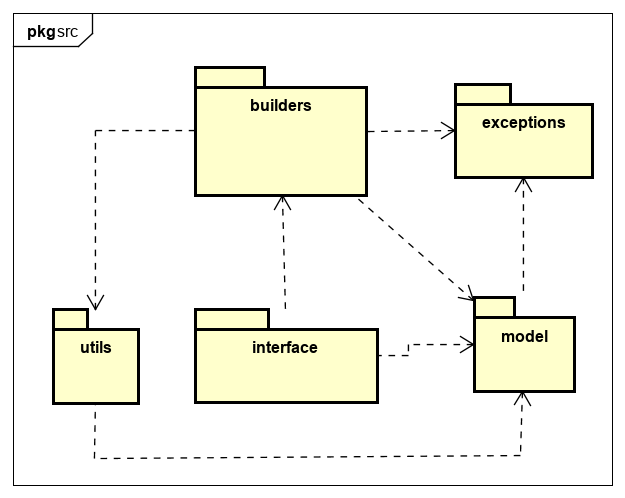
\includegraphics[width=0.7\columnwidth]{uml/packages.png} 
    \caption{Diagramma dei package}
    \label{logo:company}
\end{figure}

\subsubsection{model} %**************************
Le classi in \glsfirstoccur{model} rappresentano una configurazione \textit{NLP}.

\begin{namespacedesc}
    \classdesc{NLP}{Classe principale di \textit{model}, rappresenta una configurazione NLP. Le altre classi sono dei componenti di questa. Il metodo principale è "to\_string", che trasforma un oggetto NLP nella configurazione per \textit{Engagent}.}
    \classdesc{Rule}{Rappresenta una singola regola. Comprende il commento della regola, i \textit{match}, le domande e le risposte.}
    \classdesc{Synset}{Rappresenta un singolo synset. \'E composta da un titolo, alcuni valori di configurazione e i sinonimi.}
    \classdesc{Match}{Rappresenta un singolo match di una regola. \'E composta da un insieme di categorie, la priorità del match e un titolo.}
\end{namespacedesc}
\begin{figure}[H]
    \centering
    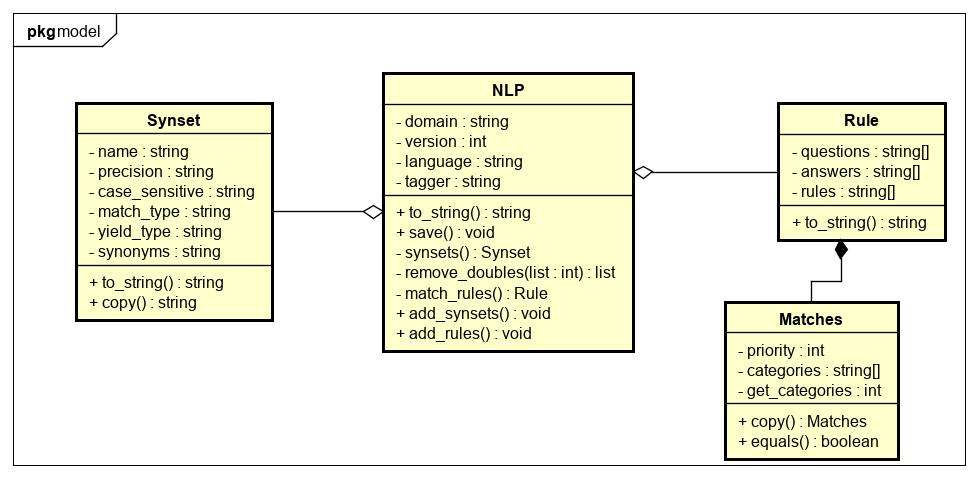
\includegraphics[width=0.7\columnwidth]{uml/model.png} 
    \caption{model}
    \label{logo:company}
\end{figure}

\subsubsection{builders} %**************************
Le classi in \textit{builders} permettono di creare un oggetto NLP, senza preoccuparsi della logica di implementazione. Attraverso il design pattern \textit{abstract method}, è possibile derivare la classe NLPBuilder, per creare builders che lavorano con formati diversi da JSON e XLSX.

\begin{namespacedesc}
    \classdesc{NLPBuilder}{Classe astratta per la creazione di un NLP. Contiene la logica principale di creazione delle configurazioni. Le classi che estendono questa classe devono solamente implementare i metodi astratti per standardizzare l'input (come definito nei commenti al codice e nel manuale dello sviluppatore).}
    \classdesc{NLPBuilderXLSX}{Classe che estende NLPBuilder. Standardizza l'input nel formato xlsx (excel).}
    \classdesc{NLPBuilderJSON}{Classe che estende NLPBuilder. Standardizza l'input nel formato json.}
\end{namespacedesc}
Nel diagramma è stato inserito anche il package \textit{model} per specificare cosa crea ogni builder.
\begin{figure}[H]
    \centering
    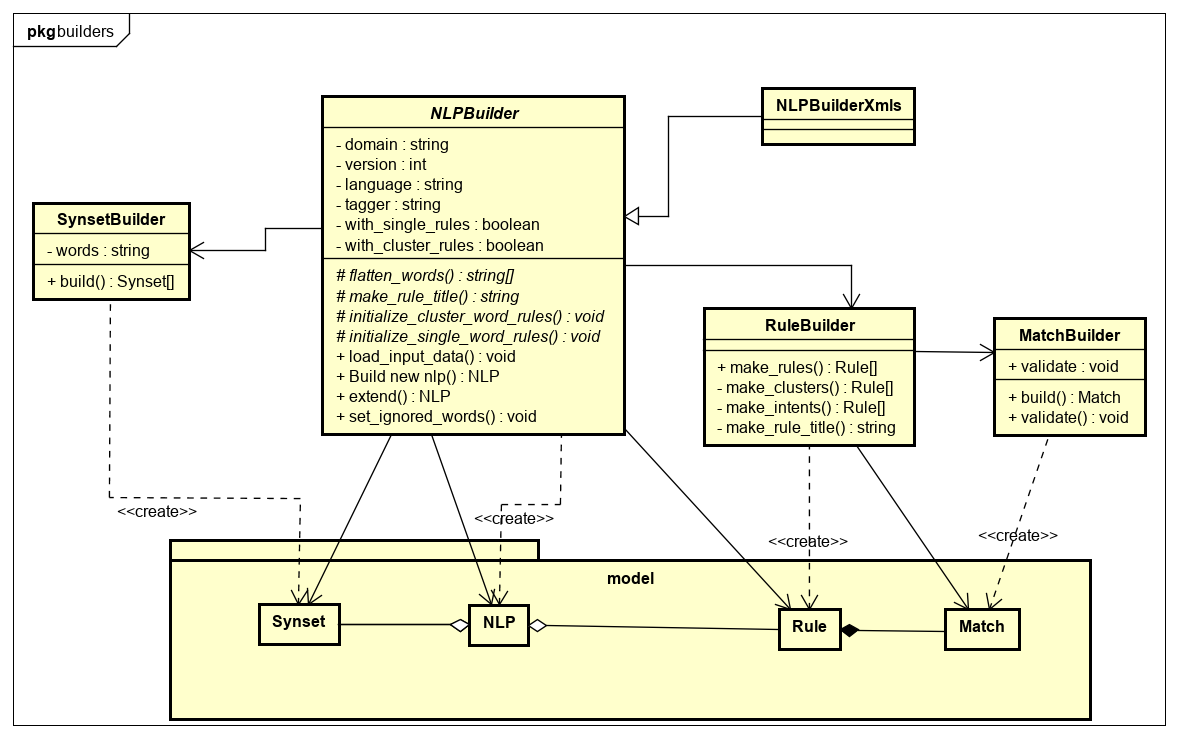
\includegraphics[width=0.7\columnwidth]{uml/build.png} 
    \caption{builders}
    \label{logo:company}
\end{figure}
\subsubsection{utils} %**************************
Contiene moduli e classi di utilità.

\begin{namespacedesc}
    \classdesc{SynsetGenerator}{Questa classe contiene la logica di \textit{business} del programma, ovvero quella che esegue la vera trasformazione dell'input in \textit{synset} e regole (a differenza del model, che si limita a tradurre tali risultati in qualcosa di compatibile con Engagent). Questa classe utilizza la libreria NLTK e TreeTagger.}
    \classdesc{Utils}{Modulo che contiene funzioni di utilità, utilizzate da più classi non dipendenti tra di loro.}
    \classdesc{NLPStemmer}{Esegue lo stemming su un oggetto di tipo NLP.}
\end{namespacedesc}
\begin{figure}[H]
    \centering
    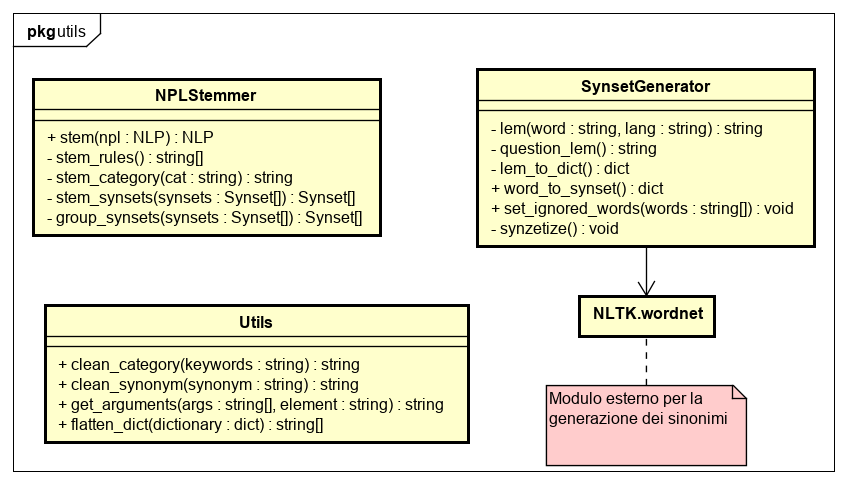
\includegraphics[width=0.7\columnwidth]{uml/utils.png} 
    \caption{utils}
    \label{logo:company}
\end{figure}
\subsubsection{interface} %**************************
Interfaccia dell'applicazione per l'utente. Permette l'interazione programmatica e a linea di comando.

\begin{namespacedesc}
    \classdesc{api}{Permette l'interazione programmatica con l'applicazione.}
    \classdesc{cli}{Permette l'interazione a linea di comando con l'applicazione.}
\end{namespacedesc}

\subsubsection{exceptions} %**************************
Eccezioni personalizzate per l'applicazione.

\begin{namespacedesc}
    \classdesc{EmptyCategoryException}{Durante l'esecuzione del programma, è stata trovata una categoria vuota.}
    \classdesc{EmptySynonymException}{Durante l'esecuzione del programma, è stato trovato un sinonimo vuoto.}
\end{namespacedesc}

%**************************************************************
\section{Design Pattern utilizzati}
L'applicazione è stata sviluppata utilizzando i seguenti design pattern:
\begin{itemize}
    \item \textbf{Builder Pattern:} la creazione di un oggetto NLP può essere complicata, perché composta da almeno quattro componenti diverse. Il builder pattern permette di semplificare questo compito, rendendo di conseguenza le classi in \textit{model} meno complesse;
    \item \textbf{Abstract Pattern:} permette di aggiungere nuovi formati in input all'applicazione senza dover riscrivere l'intera logica di creazione dell'NLP.
\end{itemize}  

%**************************************************************
\section{Codifica}
\subsection{Task della codifica}
La codifica è stata intervallata con periodi di progettazione e analisi delle nuove richieste del tutor.
Per ogni nuova componente da sviluppare, ho seguito questi passaggi:
\begin{itemize}
    \item analisi e progettazione di dettaglio del problema;
    \item ricerca di soluzioni già esistenti per questo problema;
    \item codifica di quanto progettato e sviluppo di test di unità specifici;
    \item esecuzione di tutti i test di unità e risoluzione di eventuali \textit{bug};
    \item verifica da parte del tutor aziendale;
    \item risoluzione di eventuali errori logici.
\end{itemize}

\subsection{Stile del codice}
Per facilitare il lavoro di chi dovrà manutenere il progetto, ho seguito le linee guida definite in \textit{PEP8}\footnote{\url{https://www.python.org/dev/peps/pep-0008/}} per la stesura del codice:
\begin{itemize}
    \item i metodi più significativi sono documentati con il seguente commento:
    \begin{lstlisting}
        """[Descrizione]

        Arguments:
            arg1 {[tipo]} -- [descrizione]
        Returns:
            [tipo] -- [descrizione]
        Raises:
            [exception] -- [descrizione]
        """
    \end{lstlisting}
    \item le variabili private iniziano con un doppio underscore '\_\_';
    \item le variabili protette iniziano con un singolo underscore '\_';
    \item le variabili sono scritte interamente in minuscolo, variabili composte da più parole sono seprarate da underscore (esempio: get\_name)
\end{itemize}

\subsection{Codice significativo}

Di seguito, ho riportato degli esempi di codice significativo.
\subsubsection*{Implementazione di abstract method}
L'\textit{abstract method pattern} è stato utilizzato nella classe NLPBuilder. Il ruolo dei metodi astratti è lasciare alle classi derivate il compito di implementare la logica di trasformazione dell'input in un formato standard. Questo è il minimo neccessario richiesto per implementare un nuovo builder (per un nuovo formato di input).
\newline\newline
L'implmenetazione del metodo \textit{load\_input\_data} richiede la creazione di una variabile contenente il contenuto del file di input. Questa variabile verrà utilizzata solamente dalle implementazioni degli altri metodi astratti, quindi non è predefinita.
\begin{lstlisting}[language=python]
    @abstractmethod
    def load_input_data(self, path: str):
        """load the configuration from a file

        Arguments:
            path {str} -- relative path to the file
        """
        pass
\end{lstlisting}
Il metodo \textit{\_flatten\_words} estrae le categorie dall'input definito in \textit{load\_input\_data}. Gli altri metodi astratti definiti in NLPBuilder seguono una logica simile.
\begin{lstlisting}
    @abstractmethod
    def _flatten_words(self) -> list:
        """Flatten a list of categories in the input variable defined by load_input_data.

        Returns:
            words {list} -- of categories. E.g. ['dog','cat',plain','airplain']
        """
        pass
\end{lstlisting}             % Concept Preview
% !TEX encoding = UTF-8
% !TEX TS-program = pdflatex
% !TEX root = ../tesi.tex

%**************************************************************
\chapter{Verifica e validazione}
\label{cap:verifica-validazione}
%**************************************************************             % Product Prototype
% !TEX encoding = UTF-8
% !TEX TS-program = pdflatex
% !TEX root = ../tesi.tex

%**************************************************************
\chapter{Verifica e validazione}
\label{cap:verifica-validazione}
%**************************************************************             % Product Design Freeze e SOP
% !TEX encoding = UTF-8
% !TEX TS-program = pdflatex
% !TEX root = ../tesi.tex

%**************************************************************
\chapter{Conclusioni}
\label{cap:conclusioni}
%**************************************************************

%**************************************************************
\section{Consuntivo finale}

%**************************************************************
\section{Raggiungimento degli obiettivi}

%**************************************************************
\section{Conoscenze acquisite}

%**************************************************************
\section{Valutazione personale}
             % Conclusioni
\appendix                               
% !TEX encoding = UTF-8
% !TEX TS-program = pdflatex
% !TEX root = ../tesi.tex

%**************************************************************
\chapter{Appendice A}
%**************************************************************

\epigraph{Citazione}{Autore della citazione}



             % Appendice A

%**************************************************************
% Materiale finale
%**************************************************************
\backmatter
\printglossaries
% !TEX encoding = UTF-8
% !TEX TS-program = pdflatex
% !TEX root = ../tesi.tex

%**************************************************************
% Bibliografia
%**************************************************************

\cleardoublepage
\chapter{Bibliografia}

\nocite{*}
% Stampa i riferimenti bibliografici
\printbibliography[heading=subbibliography,title={Riferimenti bibliografici},type=book]

% Stampa i siti web consultati
\printbibliography[heading=subbibliography,title={Siti web consultati},type=online]


\end{document}
